% !TEX root = ../thesis-main.tex

\chapter{Intent, Behavior and Satisfaction}
\label{chapter:research-intent}

\begin{figure}[ht]
  \centering
  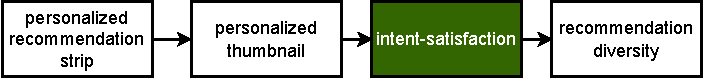
\includegraphics{images/pipeline_step3.pdf}
  \caption{The third step of the personalization pipeline}
  \label{fig:pip3}
\end{figure}

\footnote[]{This chapter was published at the ACM Transactions on Recommender Systems (TORS) under the title ``Intent-Satisfaction Modeling: From Music to Video Streaming'' \citep{intent}}
\acresetall

\if0
nth step in personalization pipeline...
motivation...
gap...
how it fits in the thesis
\fi

We are at a stage in the personalization pipeline where the platform has already nudged the user with specific content and their appearance on the page. We would like to know whether the user is satisfied with that service over time. There is a lot of research based on observable behavioral data – oftentimes aggregated over user groups – such as the time spent on the platform. But can we harness this data in a more personalized way and connect it to some latent aspects such as the users' intents and satisfaction on the platform? We reproduce a study in the music domain into the video domain at Videoland. This time, we provide all resources to reproduce our study. More precisely, we are interested in modeling the following causal chain:


\medskip
\noindent
\textbf{\ref{rq:intent}:} \acl{rq:intent}
\medskip

We answer that question for a second time, as a reproduction of a Spotify experiment~\cite{spotifyIntent}. While \cite{spotifyIntent} proposed linear logistic regression models to predict satisfaction based on intent and behavioral data, we use random forests – for higher accuracy – and hierarchical bayesian models – for better interpretability. We release simulated data, code and experimental design, to facilitate further research.

\subimport{intent-based/intentBased/sections}{01-introduction}
\subimport{intent-based/intentBased/sections}{06-related-work}
\subimport{intent-based/intentBased/sections}{02-background}
\subimport{intent-based/intentBased/sections}{03-method}
\subimport{intent-based/intentBased/sections}{04-data-analysis}
\subimport{intent-based/intentBased/sections}{05-experimental-results}
\subimport{intent-based/intentBased/sections}{07-conclusions}


\section{Upshots for the personalization pipeline}

\if0
in this chapter, ...
how we answered the research question
future work

in the next chapter we continue...
2 sentences
\fi

In this third stage of the personalization pipeline, we observe users as opposed to nudging them. Our conclusions are more mitigated than in the reproduced study~\cite{spotifyIntent} regarding the connection between intent, behavior and satisfaction data. While we are not able to reliably predict satisfaction, we are able to assess that intent influences satisfaction greatly.

Answering our research question is only possible if a platform can perform user surveys over a long period of time, collect behavioral data and connect survey and behavioral data at user-level. This step is inherent of each platform's internal organization and is an essential stepping stone. Once an organization achieves that data collection process, we hope that we can at least facilitate the rest of the process, by providing simulated data, code, experimental and survey design. Further research in that area is needed to allow to port this study to other domains like live streaming or podcasting.

In the next chapter of this thesis and the last step of our pipeline, we take a step back. This time, we use behavioral data to assess how diverse recommendations are, and how this fits to the platforms norms and values.

\section*{Reproducibility}
To facilitate the reproducibility of the work in this chapter, our code is available at \url{https://github.com/rtlnl/streaming-intent-model}.

\begin{appendices}
\chapter{Appendix of Intent, Behavior and Satisfaction}
\subimport{intent-based/intentBased/appendix}{appendix}
\end{appendices}